\section{Experiments}
% \vspace{-2mm}
\label{sec:main_expts}

We next illustrate the in-context learning abilities of the multi-trajectory transformer on unseen MiniHack and Procgen tasks, and compare against single-trajectory and hashmap-based baselines. While many previous works have studied generalization to new levels, to our knowledge we are the first to study generalization to completely different tasks, and we demonstrate promising results. 



\textbf{Baselines}: We compare against two baselines. \textbf{Hashmap (HM):} employs a hashmap over states in order to take the action corresponding to the same state from context (i.e., the expert action). It's important to note that in deterministic environments, this baseline acts as an oracle. However, in stochastic environments, it struggles to generalize to states that are not present in the demonstration. \textbf{Behavioural Cloning (BC):} trains a transformer with single trajectory sequences. BC learns a policy to predict the action the expert would take given the history of transitions so far in the current trajectory. During evaluation time, we condition BC on zero (\textbf{BC-0}) and one (\textbf{BC-1}) demonstration, respectively. Because of the lack of context, BC struggles to generalize to new tasks. 

\subsection{Main Results}
\label{sec:main_results}
\subsection{MiniHack} We collect offline data from 12 MiniHack tasks and train a multi-trajectory transformer on sequences comprising eight trajectories from the same level ($p_b = 1$). For evaluation, we test the performance on 4 new MiniHack tasks. We would like to emphasize that environments are stochastic where the stochasticity is induced by sticky actions. The results are reported in \Cref{fig:few_shot_results}. Our approach achieves good performance across multiple scenarios, demonstrating that it can learn new tasks with only a handful of demonstrations and without any weight updates. In addition, there is a consistent increase in performance with the addition of more demonstrations across all environments. Notably, our model outperforms all the baselines. When compared to BC, it underscores the significance of training transformers on sequences of trajectories, rather than on single trajectories, to foster in-context learning of new tasks. In contrast to the Hashmap, our model demonstrates the capability to learn a policy that generalizes to unseen states, rather than merely copying actions from its context which is insufficient in this setting.


\begin{figure}[t]
    \centering
    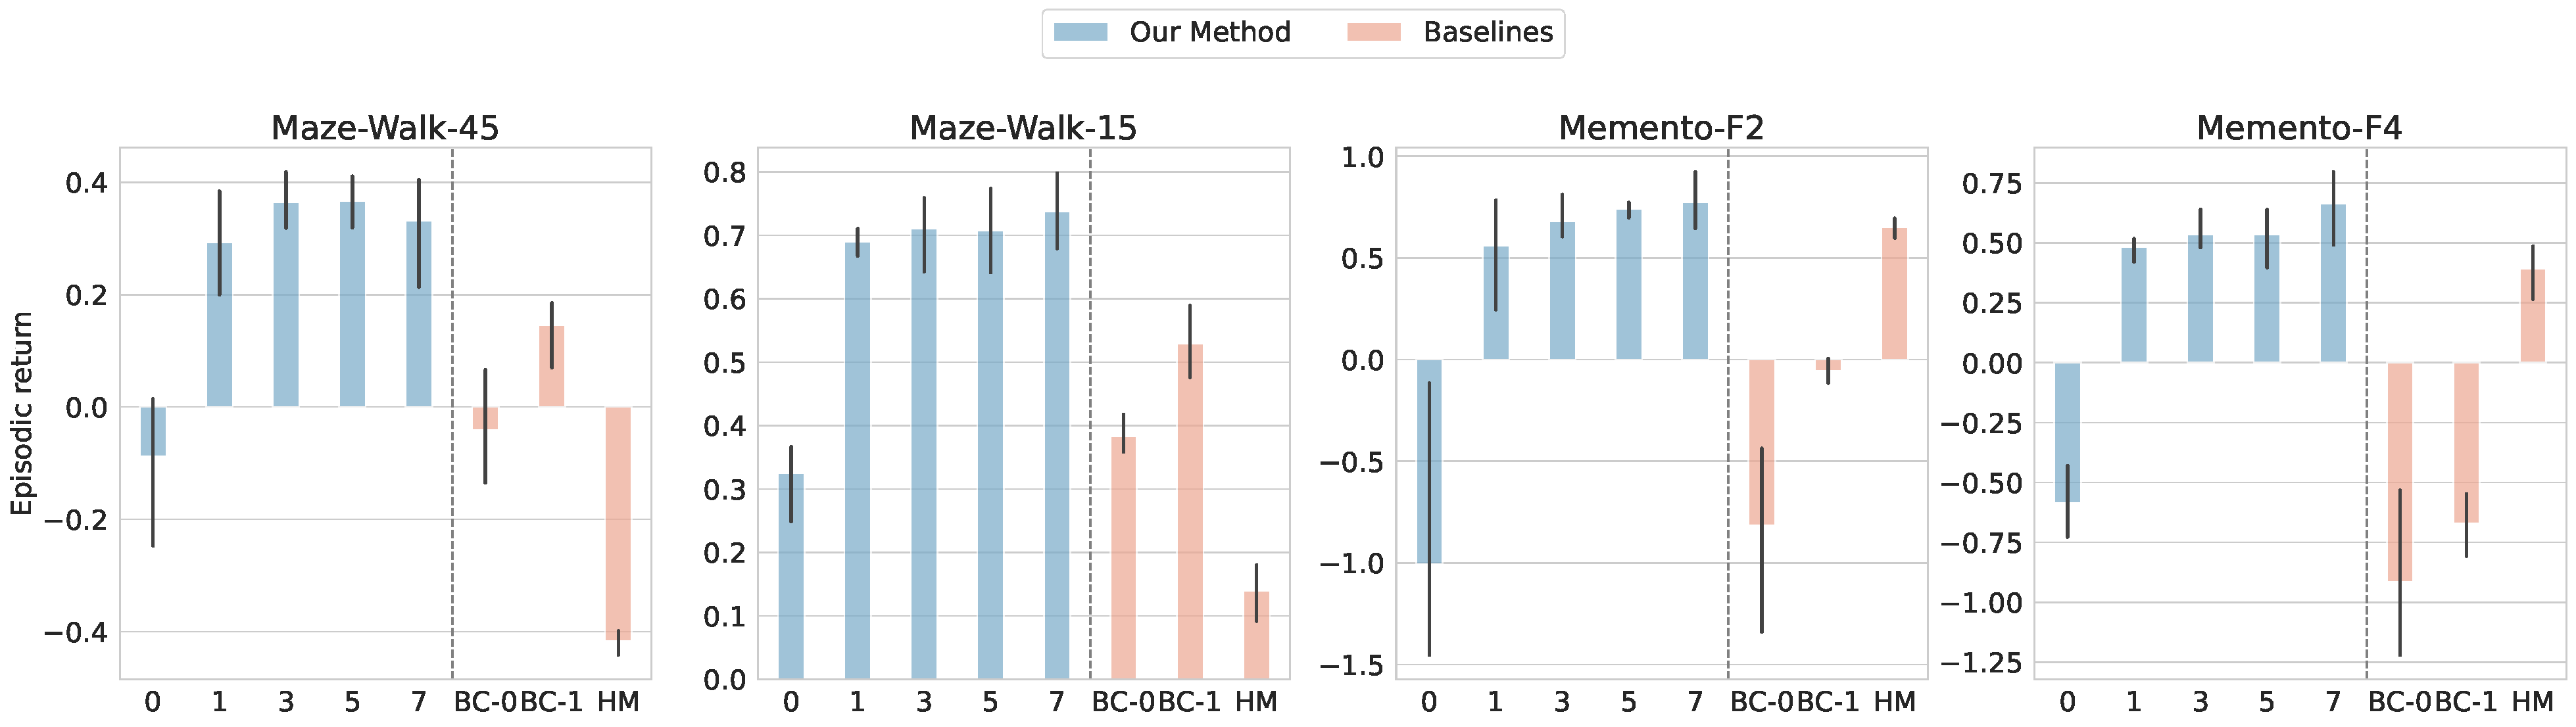
\includegraphics[width=\columnwidth]{figures/few_shot_baseline_plot.pdf}
    \caption{\textbf{Performance on New MiniHack Tasks} comparing (1) our multi-trajectory transformer conditioned on different number of demonstrations from the same level, (2) Hashmap baseline conditioned on the same demonstrations, and (3) BC baseline conditioned on zero or one demonstration due to context length constraints. Our model outperforms both baselines when provided with at least one demonstration and its performance improves with the number of demonstration. }
    \label{fig:few_shot_results}
\end{figure}


\subsection{Procgen} We also evaluate our approach on a high-dimensional pixel-based domain to test (\Cref{fig:train_test}) the generality of our findings. To do so, we collect offline data from 12 Procgen tasks and train a 310M transformer model on Procgen sequences compromising of five episodes from the same level ($p_b = 1$). We then evaluate the performance on four unseen tasks. To induce stochasticity, we use sticky actions with sticky probability 0.2 while performing online rollouts\footnote{We also vary this probability found no difference in our conclusions (\Cref{app:procgen_sticky})}. 
As shown in \Cref{fig:Procgen_results}, the performance of our model consistently increases as we condition on more demonstrations while outperforming the baselines. Finally note that it is not fair to compare our results with \cite{cobbe2020leveraging} because we only provide handful demonstrations to learn and the test tasks are disjoint from the train. 

% In the case of Maze, the improvement with number of demonstrations is not substantial. We believe this is due to the fact that in Maze, the spatial information of the agent consists of only a few pixels and hence it maybe not be captured by the visual encoder making it difficult to take good actions.

In summary, our results show that our method works well in complex pixel environments where learning good state representations is hard, and where states, layouts, dynamics, rewards, colors, textures, backgrounds, and visual features all vary between training and testing.
\begin{figure}
    \centering
    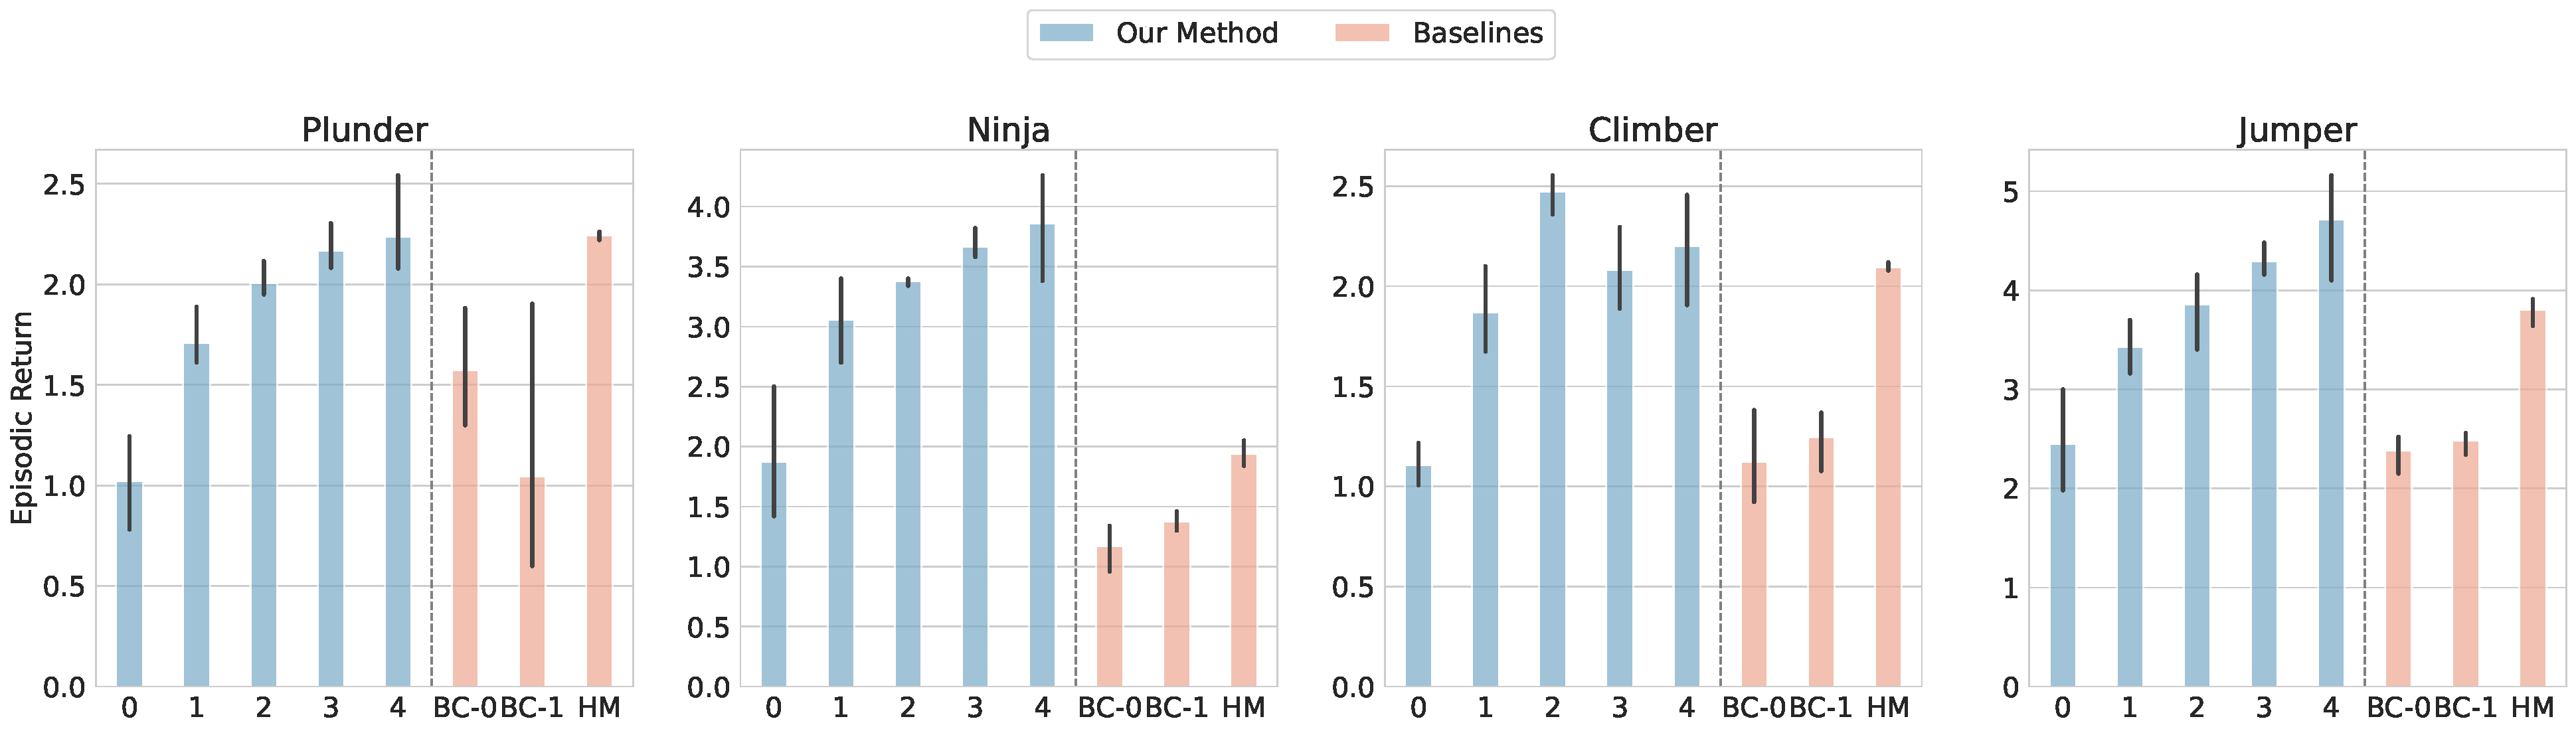
\includegraphics[width=\columnwidth]{figures/few_shot_results_procgen_1_train.pdf}
    \caption{\textbf{Performance on New Procgen Tasks} comparing (1) our multi-trajectory transformer conditioned on different number of demonstrations from the same level, (2) Hashmap baseline conditioned on the same demonstrations, and (3) BC baseline conditioned on zero or one demonstration due to context length constraints. Our model outperforms both behavioral cloning baselines, is competitive with Hashmap on Plunder, and its performance improves with demonstrations.}
    \label{fig:Procgen_results}
\end{figure}


\section{Detailed Analysis on MiniHack}
\label{sec:analysis}

\label{sec:results}
In this section, we conduct an extensive analysis on the different factors which affect in-context learning for sequential decision making. 
We highlight both zero-shot and one-shot results and conclude with a discussion on failure cases. As we've seen in the previous section, adding more demonstrations in the context generally improves the results, so here we focus on the comparison between zero-shot and one-shot which is the most significant.

\subsection{Effect of Trajectory Burstiness}
%\vspace{-3mm}
\label{sec:burstiness}
\begin{figure}[t]
    
        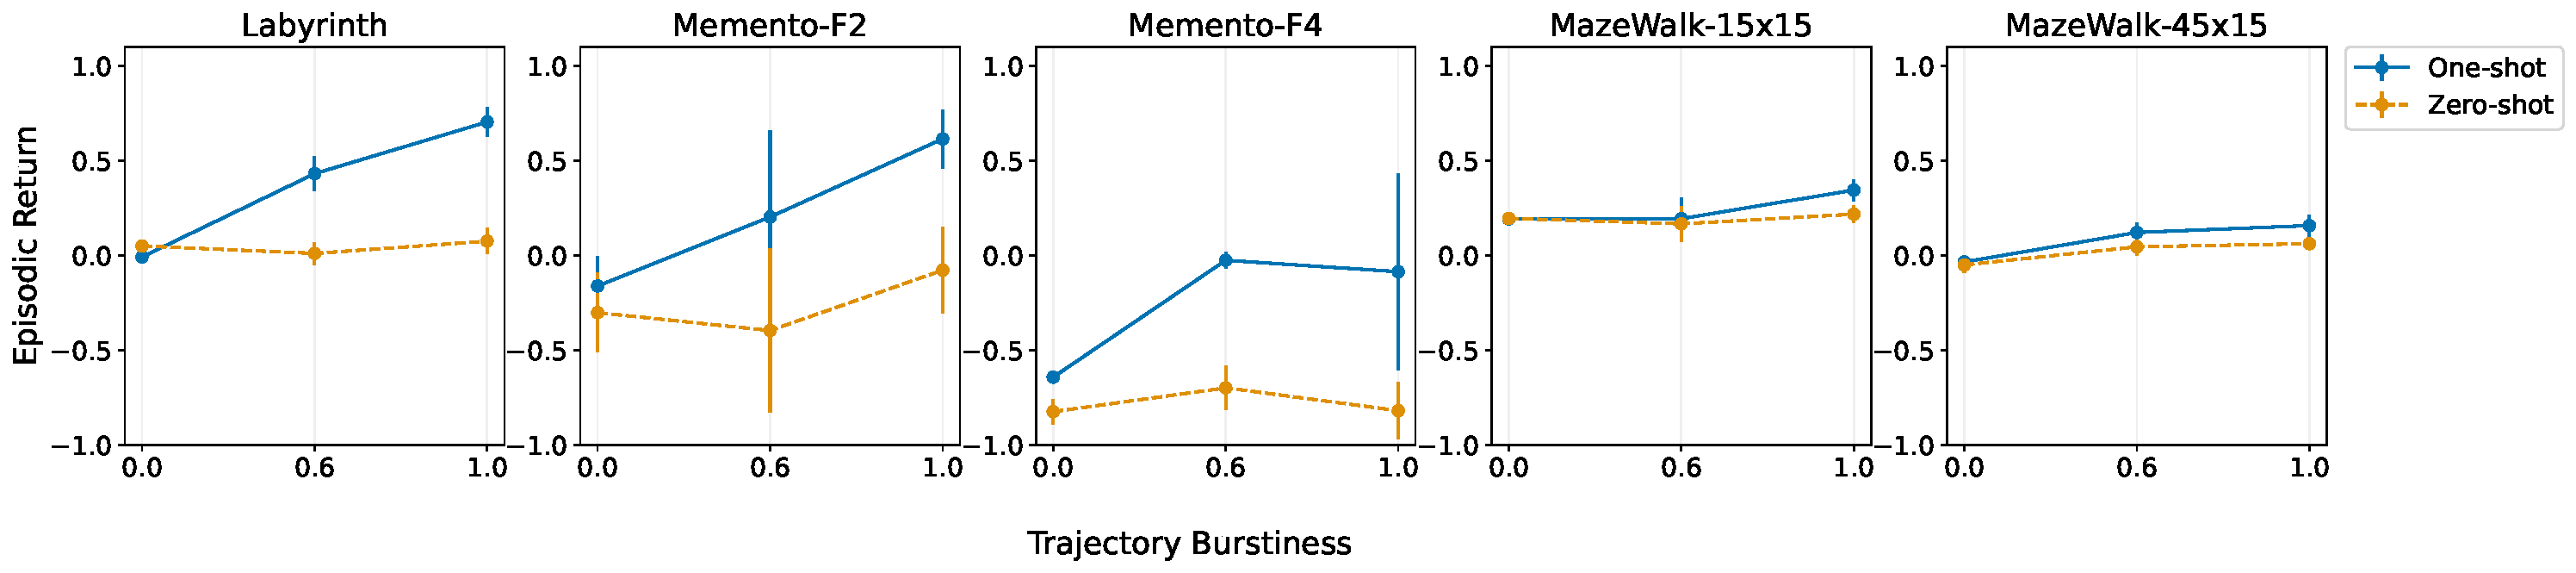
\includegraphics[width=\linewidth]{figures/burstiness_12_envs.pdf}
        \caption{\textbf{Effect of Trajectory Burstiness}: Mean performance (with std. across $3$ seeds) for different levels of trajectory burstiness (a), dataset sizes (b), model sizes (c) and numbers of training tasks (d). These factors all have a positive effect on in-context learning.}
        \label{fig:burstiness}
\end{figure}
\begin{figure}[t]
    \centering
    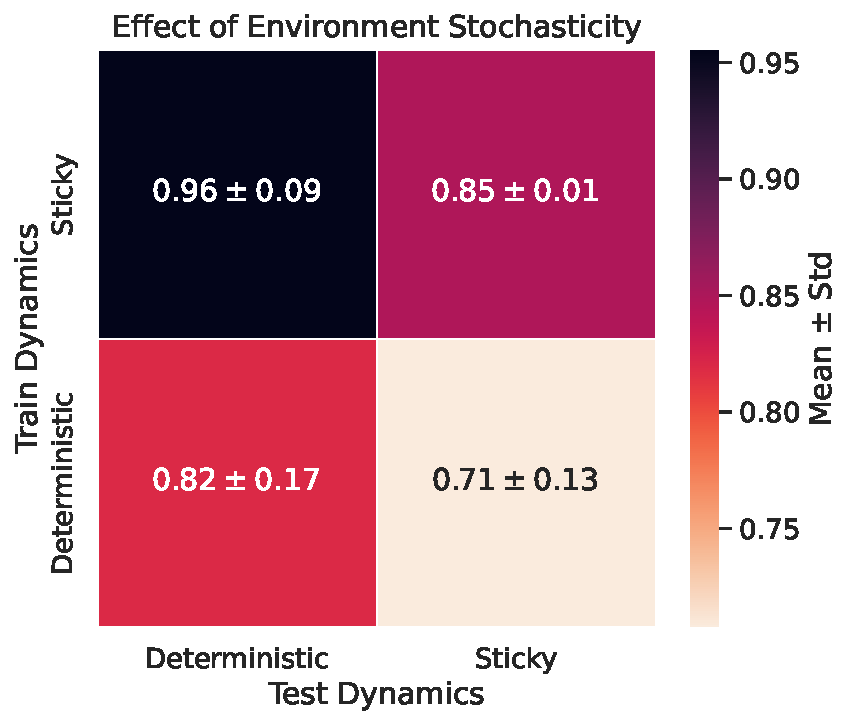
\includegraphics[scale=0.5]{figures/env_dynamics.PDF}
    \caption{\textbf{Effect of Environment Stochasticity:} This figure illustrates the effect of environment dynamics on in-context learning of Labyrinth task. The x-axis denotes the environment dynamics considered during evaluation and the y-axis denotes the environment dynamics used for training. The numbers and heatmap colors indicate the one-shot performance, capturing the mean and standard deviation of episodic returns across 3 model seeds. 
    }
    \label{fig:env_dynamics}
\end{figure}
First, we analyze the effect of trajectory burstiness. 
We hypothesize that having demonstrations similar to the query inside the context (\ie{} trajectory burstiness) encourages the model to utilize the contextual information. 

Our results in \Cref{fig:burstiness} confirm that in-context learning improves with more trajectory burstiness, resulting in strong one-shot generalization to new tasks for $p_b = 1$. This is consistent with insights from supervised learning~\cite{zipfian_icl}. 

\subsection{Effect of Environment Stochasticity}
%\vspace{-3mm}
\label{sec:env_stochasticity}


    
We next investigate the impact of different environment dynamics on in-context learning. For this, we gather offline data using expert E3B policies in both deterministic and stochastic environments. To introduce stochasticity in the environments, we employ sticky actions, a widely utilized technique in deep reinforcement learning~\citep{machado2018revisiting} where previous actions are repeated with some probability ($p=0.1$ in our experiments). 

We gather pretraining datasets from both stochastic and deterministic versions of the \texttt{MiniHack-MultiRoom-N6} task, which we use to train two separate variants of the transformer model. We then evaluate each model on unseen environments with either stochastic or deterministic dynamics. Results are shown in a confusion matrix in \Cref{fig:env_dynamics}. 

Models trained with stochastic dynamics exhibit superior performance on unseen tasks, whether their dynamics are deterministic or stochastic. 
An explanation is that when dynamics are deterministic, the diversity within the training dataset is comparatively low, resulting in identical copies of the trajectory in the context and query. This limits the model's in-context learning ability to pure copying behavior. In contrast, when the training environment dynamics are stochastic, the pretraining dataset exhibits greater diversity and identical copies of the trajectory become rarer, forcing the model to generalize from similar, but not identical, trajectories. 


\subsection{Effect of Dataset Size}
%\vspace{-2mm}
\label{sec:dataset_size}

    \begin{figure}[t]
        \centering
        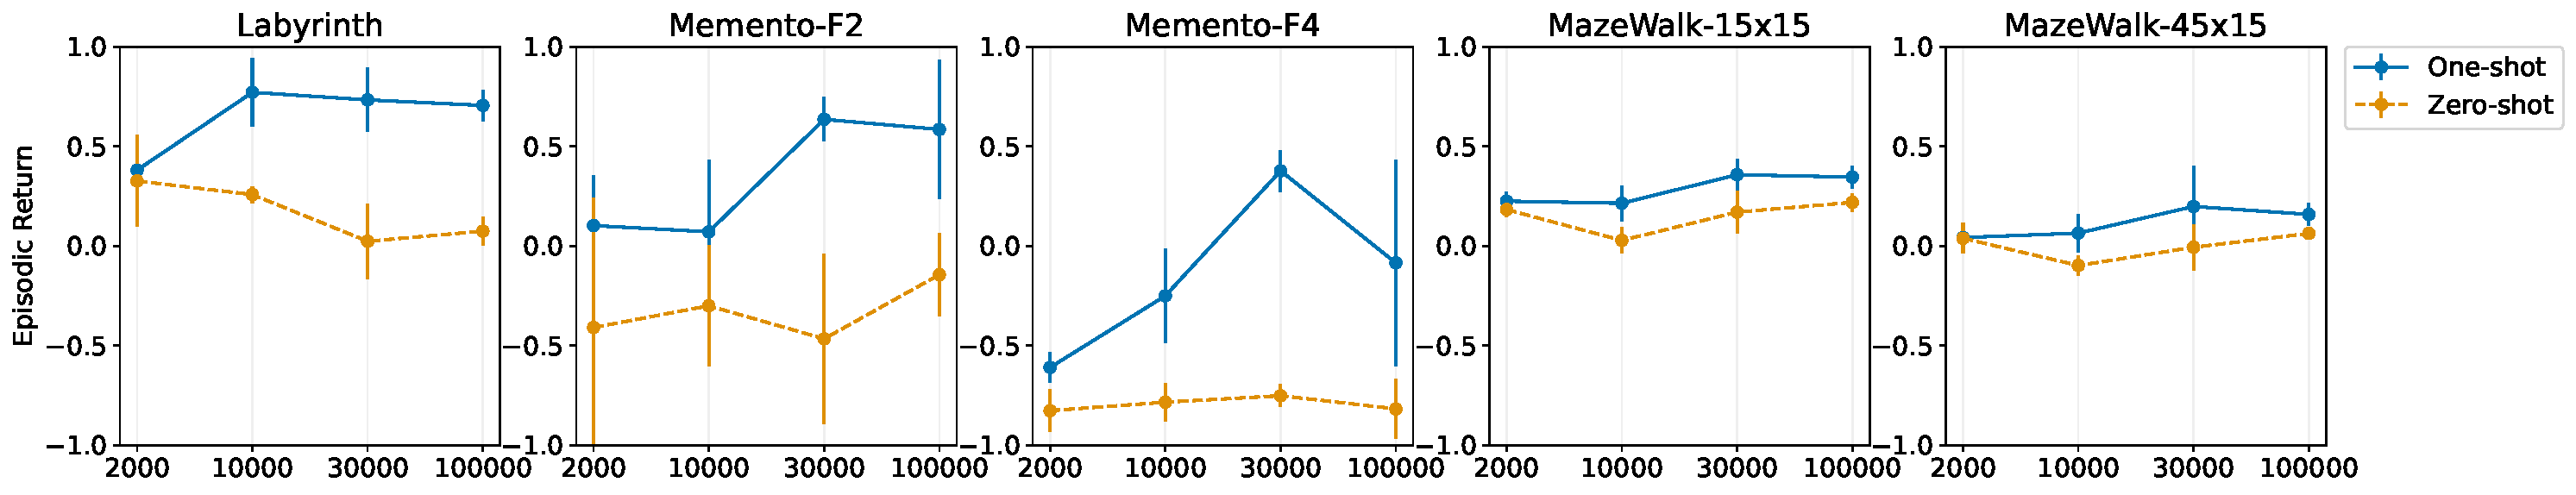
\includegraphics[width=\linewidth]{figures/dataset_scaling_v2.pdf}
        \caption{\textbf{Effect of Dataset Size}: This figure illustrates the effect of the dataset size on the average episode return for 5 unseen MiniHack tasks. The dashed line indicates the zero-shot performance, and the solid line represents the one-shot performance. Overall, both the one-shot performance improves when increasing the dataset size from 2k to 30K levels and then they plateau. This suggests that increasing the dataset size can help both in-context learning but the improvements have diminishing returns beyond certain threshold because of lack of diversity in the training samples. The error bars represent the standard deviation across 3 model seeds.}
        \label{fig:data_scale}
    \end{figure}
    
    % \vspace{1em} % Space between subfigures
    
    \begin{figure}[b]
        \centering
        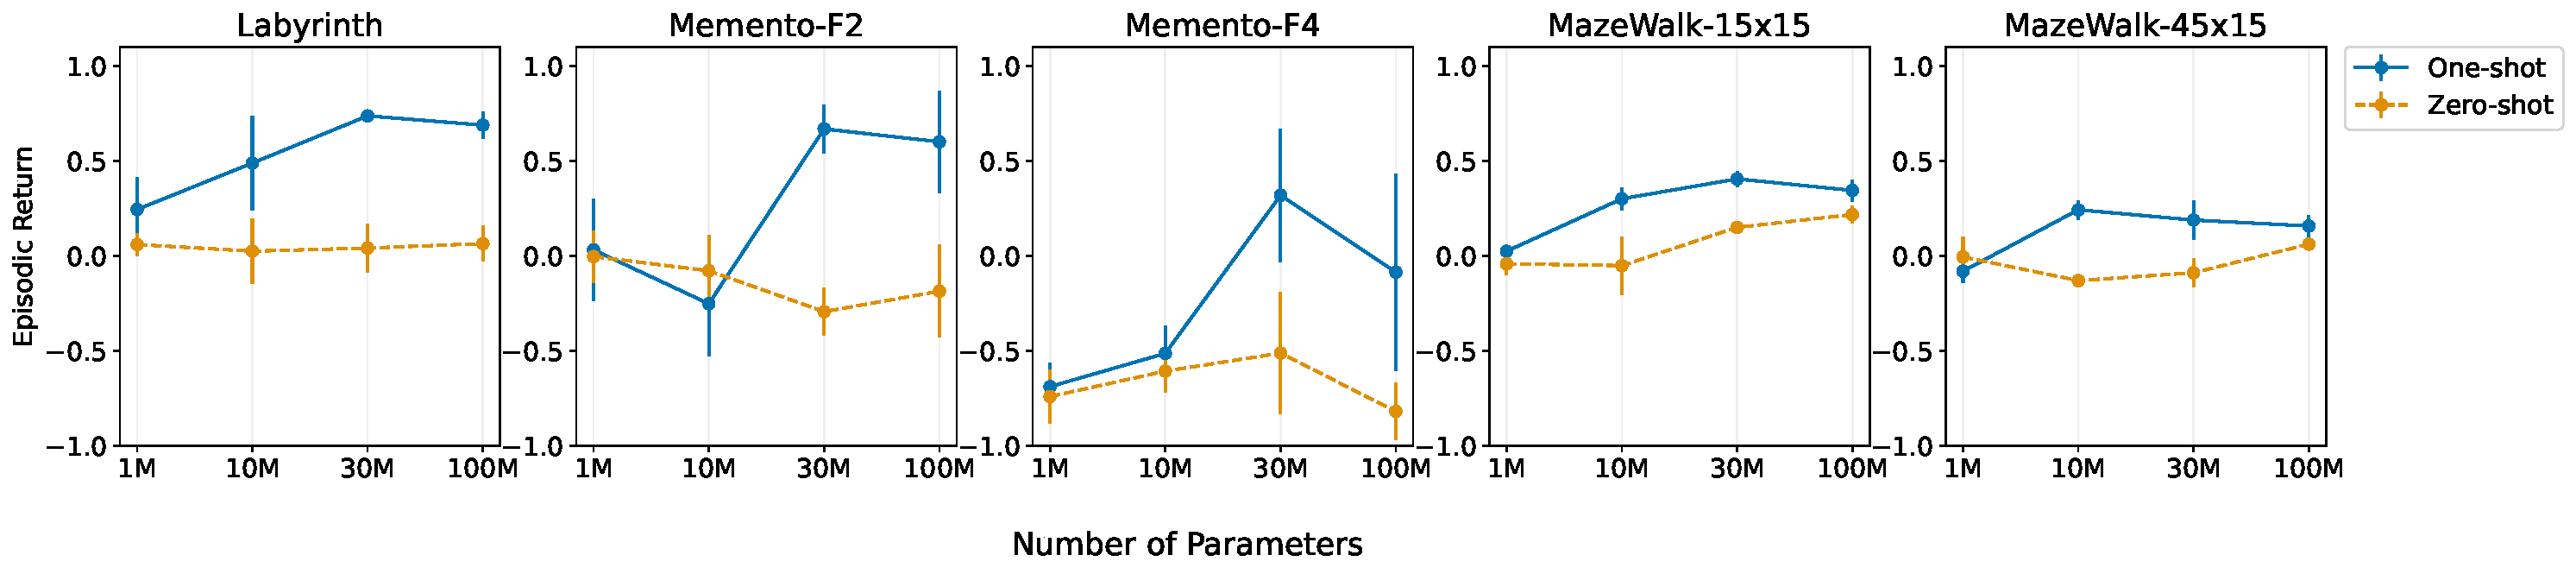
\includegraphics[width=\linewidth]{figures/model_scaling.pdf}
        \caption{\textbf{Effect of Model Size}: This figure illustrates the effect of the model size on the average episode return for 5 unseen MiniHack tasks. The dashed line indicates the zero-shot performance, and the solid line represents the one-shot performance. As the model size increases, one-shot performance consistently improves up to 30M parameters and then the performance plateaus. In contrast, the zero shot performance doesn't change as much with the number of parameters, suggesting that the model's in-context learning ability scales better than its in-weights ones with the model size. The error bars represent the standard deviation across 3 model seeds.}
        \label{fig:model_scale}
    \end{figure}
    
    % \vspace{1em} % Space between subfigures
    
    \begin{figure}[t]
        \centering
        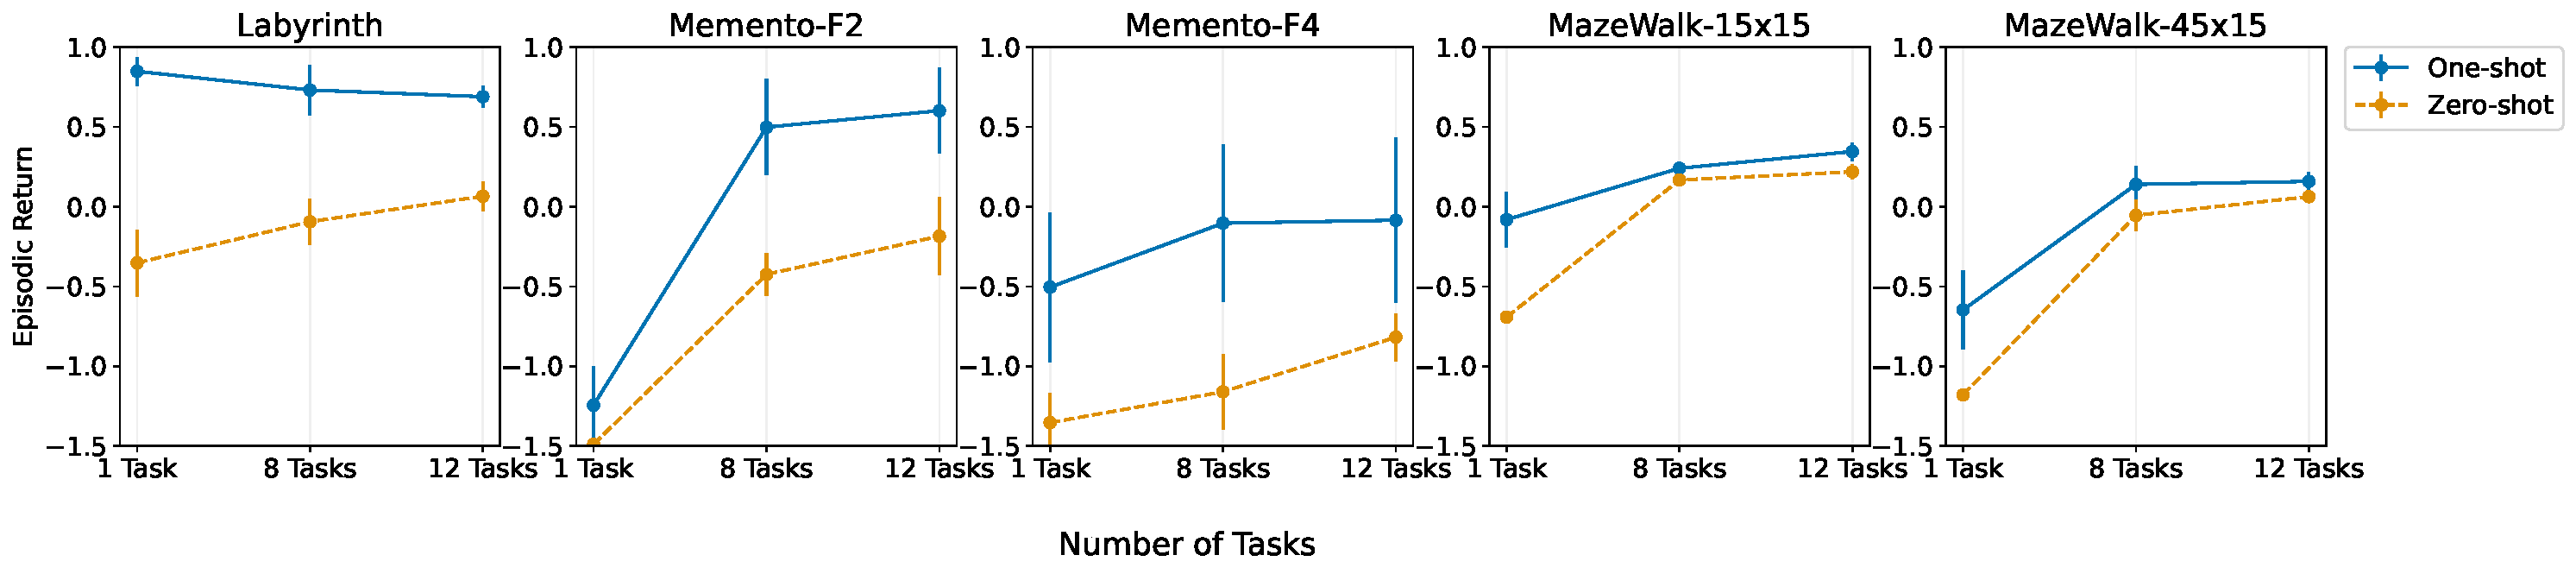
\includegraphics[width=\linewidth]{figures/env_scaling.pdf}
        \caption{\textbf{Effect of Task Diversity}:  This figure illustrates the effect of the number of different training tasks on the average episode return for 5 unseen MiniHack tasks. The dashed line indicates the zero-shot performance, and the solid line represents the one-shot performance. Overall, both the one-shot and zero-shot performances improve when increasing the number of tasks from 1 to 8, but then they plateau. This suggests that increasing the task diversity can help both the in-weights and in-context learning but the improvements have diminishing returns and may depend on the similarity between the train and test tasks. The error bars represent the standard deviation across 3 model seeds.}
        \label{fig:task_diversity}
    \end{figure}
    
    % \caption{
    % %\textbf{
    % Mean performance (with std. across $3$ seeds) for different levels of trajectory burstiness (a), dataset sizes (b), model sizes (c) and numbers of training tasks (d). These factors all have a positive effect on in-context learning.

    % }
    % \label{fig:data_scaling}

 While many studies in NLP \citep{gpt3, scaling-laws, olsson2022incontext} have reported a positive correlation between dataset size and ICL, few have studied it the realm of sequential decision making~\citep{adaptiveagentteam2023humantimescale}. Consequently, here we explore the impact of the dataset size on ICL and cross-task generalization.  We train models on varying numbers of levels from the same MiniHack task and evaluate them on a different MiniHack task. As seen in~\Cref{fig:data_scale}, performance on unseen tasks increases with the dataset size and saturates at 30K levels for one-shot models.  This is expected as the models improve on their ability to generalize as the dataset increases, even to these new tasks. Moreover, as the dataset sizes increases, we also see the emergence of a performance gap between one-shot and zero-shot evaluations on these new tasks, demonstrating the emergence of in-context learning. We also observe  that the performance saturates and subsequently increasing the dataset size above a certain scale (30K levels) yields diminishing returns. We hypothesize that this could be due to insufficient data diversity. 

\subsection{Effect of Model Size} We next scale the number of model parameters and study how it affects ICL. We evaluate transformer models with 1M, 10M, 30M and 100M parameters, trained on a dataset consisting of 100, 000 levels from 12 different MiniHack tasks. \Cref{fig:model_scale} shows that increasing the model size increases ICL on unseen tasks. However, in this case, scaling the model size has diminishing returns and the performance plateaus after 30M parameters. 

\subsection{Effect of Task Diversity} In this section, we study how ICL behaves as we scale the diversity of tasks used for training. Increasing the diversity of tasks should improve the generalization of the in-weights learning, but its not clear how this should affect a model's ability to 'soft-copy' with ICL.  In \Cref{fig:task_diversity} we see that above a certain diversity of tasks, ICL ability plateaus, while as the task diversity shrinks, some novel tasks are capable of demonstrating ICL, while others are not.  In \Cref{sec:env_difficulty}, we investigate the difference between these environments detail. 
%\vspace{-5mm}
\subsubsection{Investigating Failure Modes}
\vspace{-1mm}
% \subsection{Investigating Task Environments}
\label{sec:env_difficulty}

In this section, we aim to better understand why our approach performs much better on some tasks than others. To do so, we plot the episodic return and in-context action accuracy for 8 unseen test tasks after training the model on 12 different tasks (see \Cref{fig:failure_analysis}). The in-context action accuracy is defined as the percentage of correct actions taken by the agent (\ie{} matching the actions provided in the context corresponding to the same states). High in-context action accuracy indicates that the model is able to effectively utilize the demonstration provided in its context. 
We categorize these results into four categories, each explaining a different learning phenomenon. 

\textbf{In-Context Learning:} In this category, we have environments like \texttt{Labyrinth} and \texttt{Memento F2} with both high episodic return and high in-context action accuracy. The high in-context action accuracy indicates that the transformer learns to copy the correct action when it encounters states that appear in the given demonstration, which in turn leads to good performance on the task, as expected.

\textbf{In-Weights Learning:} In this category, we have environments like \texttt{MazeWalk-15} and \texttt{MazeWalk-45} where the episodic return is relatively high but the in-context action accuracy is low. This means that the agent manages to perform well on the new task even without copying actions from its context. This suggests the model is leveraging information stored in its weights during training, also referred to as in-weights learning~\citep{zipfian_icl}. It is worth noting that $\texttt{MazeWalk-9}$ is one of the training environments, which shares similarities with the two test ones. However, note that the test tasks are much harder versions of the training one, so they require some degree of generalization. 

\begin{figure}{b}
\centering
    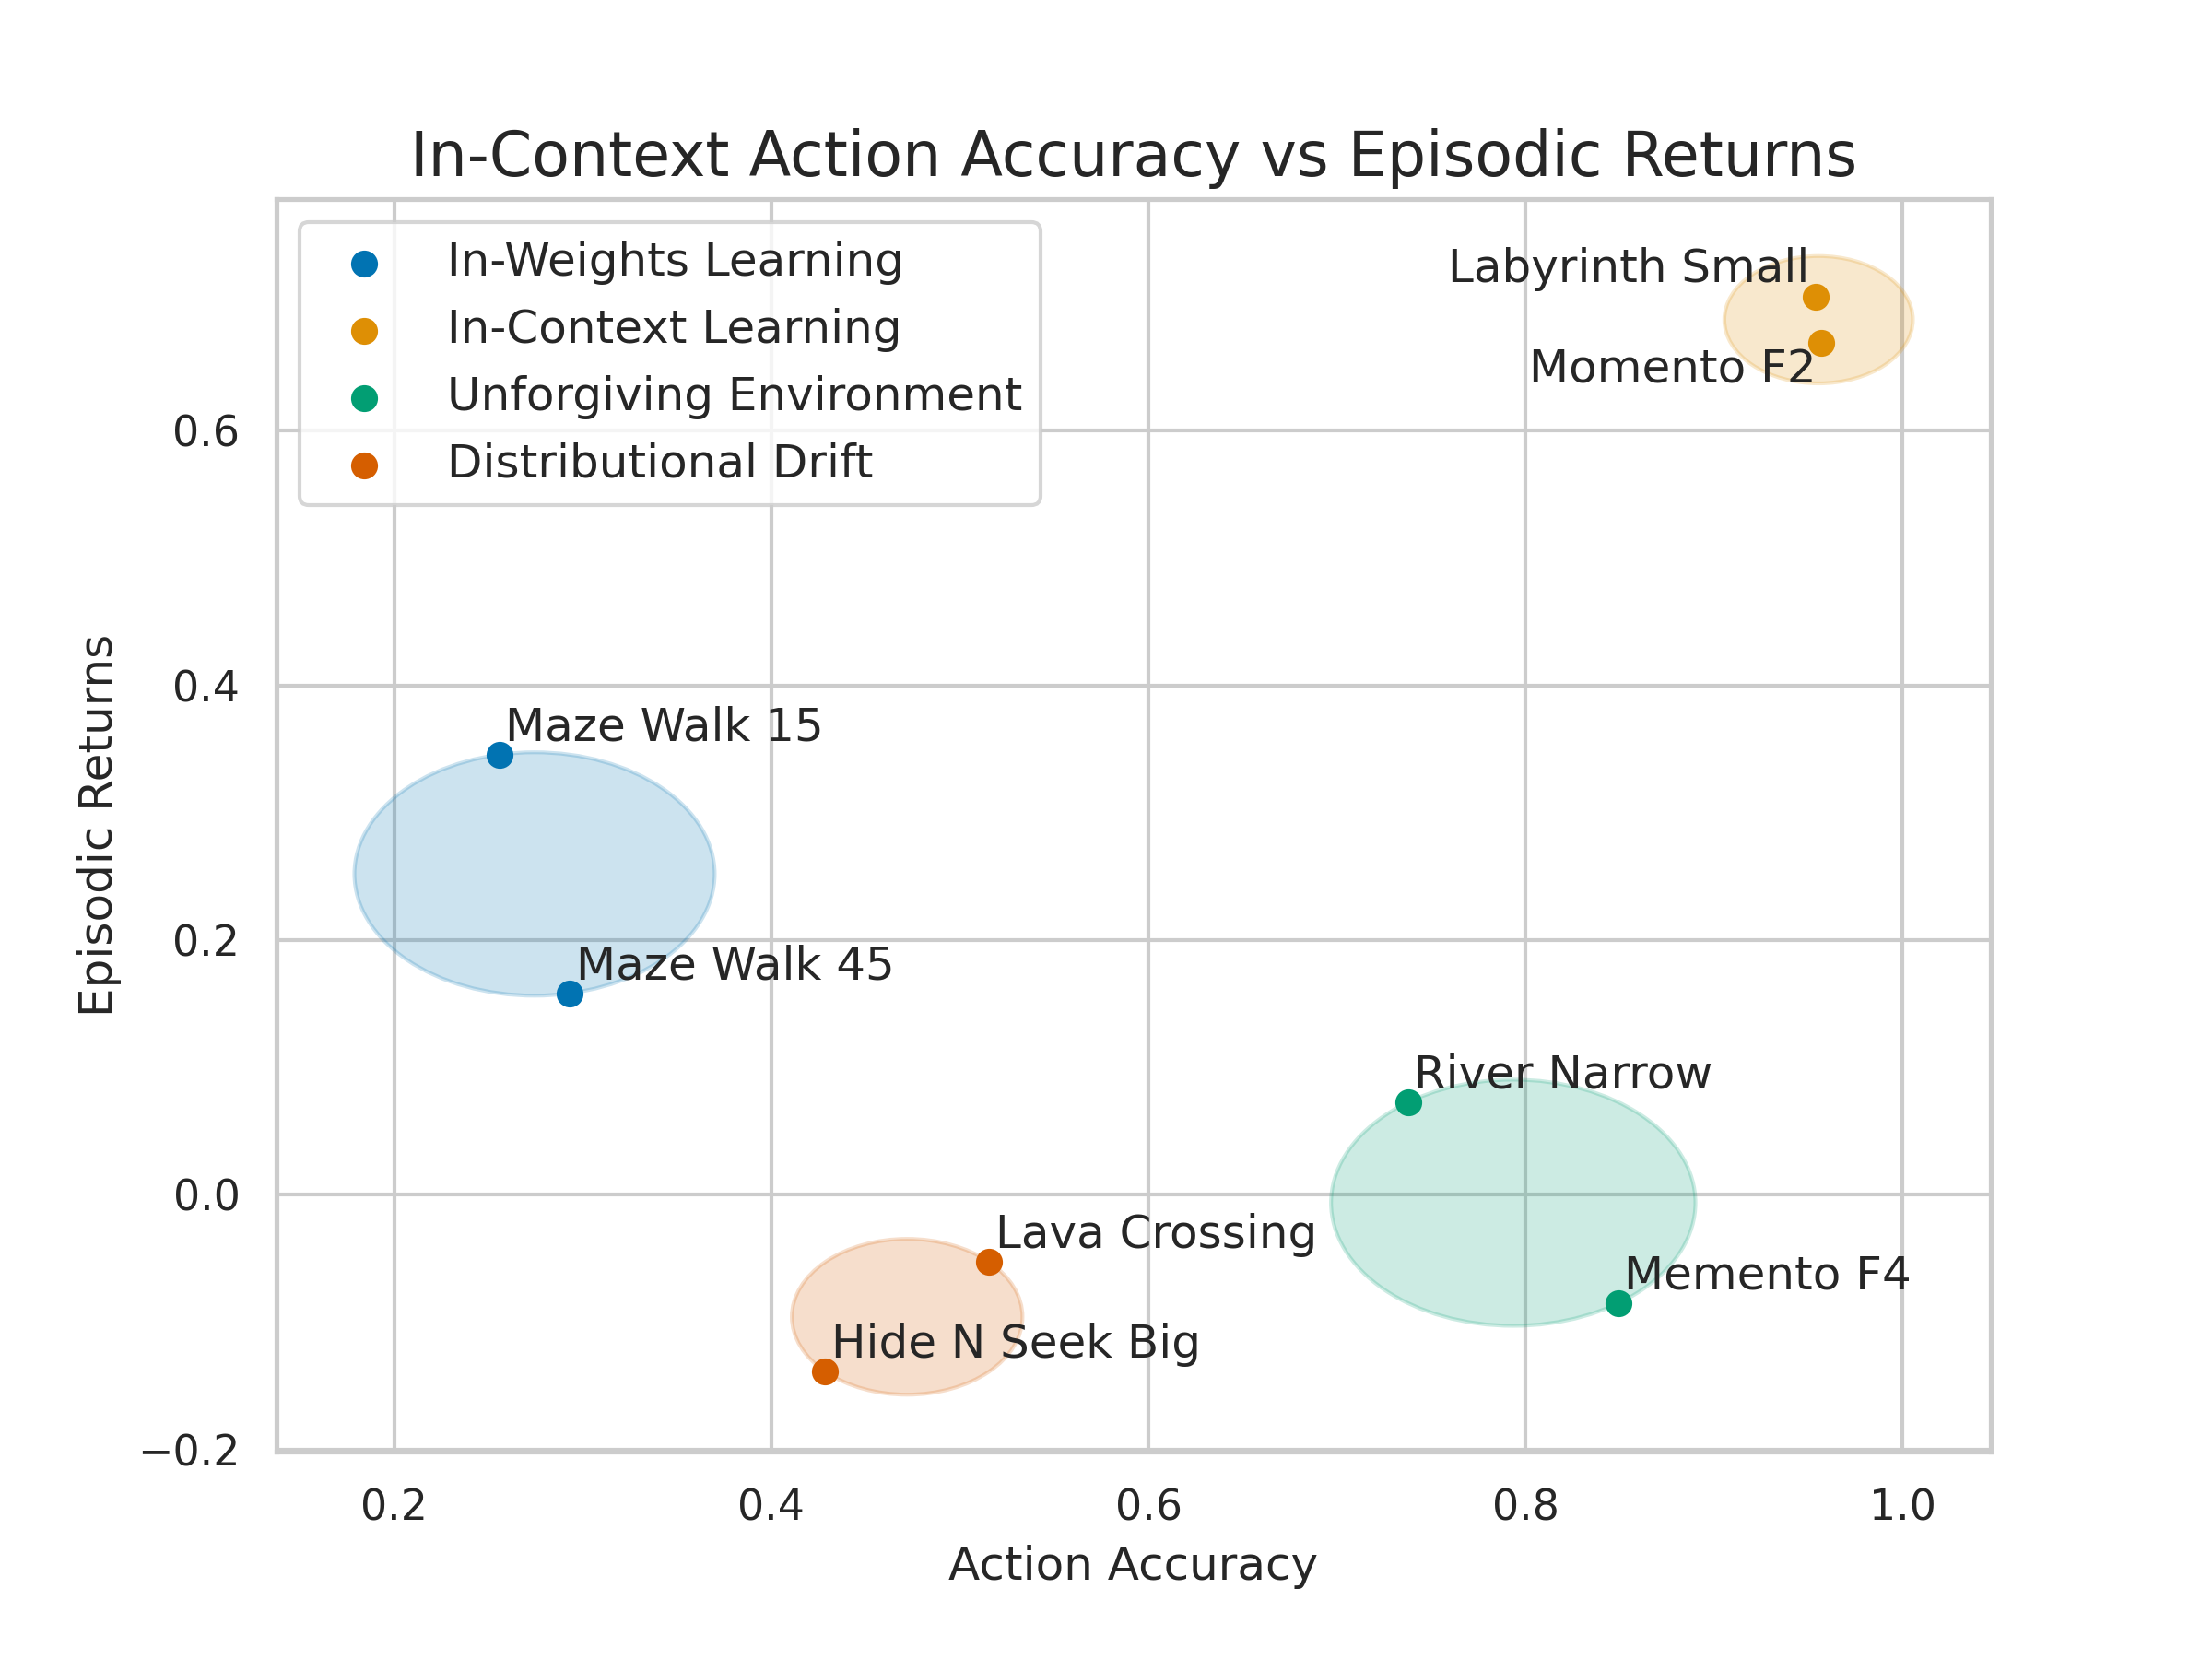
\includegraphics[width=0.5\columnwidth]{figures/failure_analysis_action_accuracy.png}
    \caption{\textbf{Investigating Failure Modes:} This figure illustrates different learning phenomena across eight tasks. The x-axis represents the in-context action accuracy, while the y-axis represents the episodic return, with each point in the plot corresponding to an unseen task. We cluster these data points using k-means clustering and color-code each cluster. Each cluster corresponds to a different learning phenomenon, which are discussed in-depth in \Cref{sec:env_difficulty}.}
    \label{fig:failure_analysis}
\end{figure}
\textbf{Unforgiving Environment:} This category includes environments such as \texttt{River-Narrow} and \texttt{Memento-F4} with high in-context action accuracy but low episodic returns. This indicates that while the agent is able to perform in-context learning and predict the correct action for most states that appear in the demonstration, it still cannot achieve high reward due to reaching unrecoverable states.
%(\eg{} where the episode ends without reward). 
This is reminiscent of the covariate shift problem in imitation learning, where despite predicting actions well on the expert data, the agent performs poorly at deployment due to small mistakes which put it outside the training distribution~\citep{ross2011reduction}. 



\textbf{Distributional Drift:} In the last category, we have environments like \texttt{Lava-Crossing} and \texttt{Hide-N-Seek-Big} where both the episodic return and the in-context action accuracy are low. Here, the agent is unable to perform in-context learning and the test tasks are too different from the training ones for in-weights learning to be effective.